%%%%%%%%%%%%%%%%%%%%%%%%%%%%%%%%%%%%%%%%%%%%%%%%%%%%%%%%%%%%%%%%%%%%%%%
%%%                           SECTION II
%%%%%%%%%%%%%%%%%%%%%%%%%%%%%%%%%%%%%%%%%%%%%%%%%%%%%%%%%%%%%%%%%%%%%%


\chapter{METHODOLOGY}
% Our preliminary results consist of an evaluation of pixel distribution distances as an effective metric, as well as the exploration of other image features to be used in our learning algorithm.
% In our prelimiary analysis we had access to a small dataset; we have recently gained access to a much larger dataset which we are currently cleaning and labeling in order to further our training and analysis.
% This analysis was performed on greyscale images, as we did not yet have access to images with many bands, and greyscale or average intensity values have traditionally proven to be effective for image analysis.

Our methodology for this research consists of several steps.
First, the larger data archive is accessed; and the datasets, selected.
Next, the data is cleaned, and labeled according to our criteria.
Once the data is prepared, we perform feature evaluation: the process of extracting image features and analyzing them for their potential use in learning algorithms to detect anomalous images.
Various distance metrics are then calculated, and again these metrics are analyzed for their utility in distinguishing acceptable images from anomalous ones.
Finally, these metrics for each pair of consecutive images are concatenated, along with the previously generated labels, and used as training data in our learning algorithms.
Beyond this, various synthetic features are generated, and the parameters of the learning models are adjusted to achieve optimal results.


\section{Data Preparation}

To obtain usable datasets for training and testing, we first access the raw data.
Once imaging flights run by the Texas A\&M GEOSAT group are completed, the raw data is pushed to a network drive.
The data is ordinarily then accessed by another member of the GEOSAT group, who performs orthomosaicking to produce a single map of the target area.
As stated in the problem formulation, this raw data generally contains images which are problematic, i.e., the camera was not pointed normally towards the ground, and thus the images are not reconcilable with respect to the surrounding images.
Our goal in selecting data from the source is to find datasets over unique areas which are sufficiently large, generally more than 1000 usable images, and which have a sufficient percentage of anomalous images.

The data selection yielded four large datsets, totalling 8768 images.
Since the current imaging process has the camera taking images before and during takeoff, as well as during and after landing, these images have to be identified and removed.
After this initial data cleaning, our datasets totalled 4863 images.
The images are then searched through manually in order to create a list of anomalous image names which can later be used to generate label vectors for training and testing.
After this process, 244 anomalous images were discovered among the four datasets, achieving a target rate of roughly 5\%.

Finally, in accordance with most image processing standards, the images are all converted to grayscale.
There are a few reasons for this: the first is that luminence (i.e., the grayscale values from a color image) is revealing enough for the vast majority of image processing task; a secondary reason is to ease processing time by cutting the data processing by 2/3, which is particulary important to our application.


\section{Image Feature Evaluation}

In this problem, we wish to find a set of features that can be quickly extracted from images, and used to train a model to identify images that do not belong in the stream.
The first step in this process is to evaluate features to find ones that are suitable to our needs: quickly extracted and sufficiently distinguishing between overlapping and non-overlapping images.

Several types of image features are explored for this purpose.
Pixel distributions, binary features, local binary patterns, and blob detection were all extracted for a subset of the overall dataset and evaluated for their efficacy.
Once image features are extracted, a few distance metrics are applied to compare the features between consecutive images.
The distances are then compared between instances of acceptable pairs of images and pairs which contain anomalies to determine if the feature is usable.


\subsection{Distribution Distances}

When thinking of the differences between overlapping and non-overlapping images, pixel distribution was one of our first ideas.
Pixel distribution is a very simple feature to extract: it can be done in linear time with respect to the number of pixels, and is easily distributable.
Furthermore, it is clear that images with a large overlap will have fairly similar pixel distributions (since much of their conent is nearly identical), and non-overlapping images may be dissimilar.

Once pixel distributions are extracted, a method for comparing the distributions is needed.
From the field of statistics, there are a few methods for calculating ``distances'' between distributions: the higher the distance, the less similar the distributions are in some way.

The first distance metric we looked at is a very common method for calculating the distance between two sets of numbers: the mean-squared error or MSE.
Essentially, the MSE is the L-2 norm of the errors or differences between the two sets of numbers.
If we consider the vector $\underline{\mathbf{p}}$ to be one distribution and the vector $\underline{\mathbf{q}}$ to be another distribution, each of length $n$, then the MSE is given by:
\begin{equation}
\frac{1}{n} \left( \sum_{i=1}^n{(p_i-q_i)^2} \right)^{1/2} .
\end{equation}

While the MSE does provide a distance between the two distributions, it is more suited to calculating errors, as the name suggests.
Another distance metric, called the Bhattacharyya distance, is actually designed to measure the similarity between two continuous or discrete probability distributions.
It is calculated by taking the negative of the log of the closely related Bhattacharyya coefficient.
The Bhattacharyya coefficient was designed to be a metric for the amount of overlap between two distributions, defined as:
\begin{equation}
BC(\mathbf{p}, \mathbf{q}) = \sum_{i=1}^n{\sqrt{p_iq_i}} .
\end{equation}
Making the Bhattacharyya distance equal to:
\begin{equation}
BD(\mathbf{p}, \mathbf{q}) = - \ln \left( \sum_{i=1}^n {\sqrt{p_iq_i}} \right) .
\end{equation}

Another potential distance metric for distributions is the Earth Mover's Distance (EMD), known in mathematics as the Wasserstein metric.
If the distributions are considered to be two different ways of arranging piles of mass, then the EMD gives the minimum amount of mass that needs to be moved times the distance it is moved in order to turn one set of piles into another.

Formally, the EMD is defined as the solution to:

XXX

subject to 

XXX


The results were predictably better using the Bhattacharyya distance rather than the MSE and Earth Mover's Distance, so this distance metric was used for evaluation of distributions as a distinguishing feature.
It is worth noting that the Bhattacharyya distances are calculated in linear time with respect to the number of possible intensity values.


% \subsection{Application to images with peak-finding}

% In order to evaluate the effectiveness of the Bhattacharyya distance as a distinguishing feature, we calculated the distance between distributions of consecutive images in our datasets.
% Even between the two flights contained in our dataset, the means and variances between flights were widely different, making a simple threshold invalid as a classifier.
% Instead, we considered the distance values as a signal and used the peak-finding capabilities in SciPy to correlate spikes in the distances with the anomalous images we are trying to detect.

% Below are two figures showing the distance metrics of our two flights with the detected peaks marked:

% \begin{figure}[h]
% \centering
% 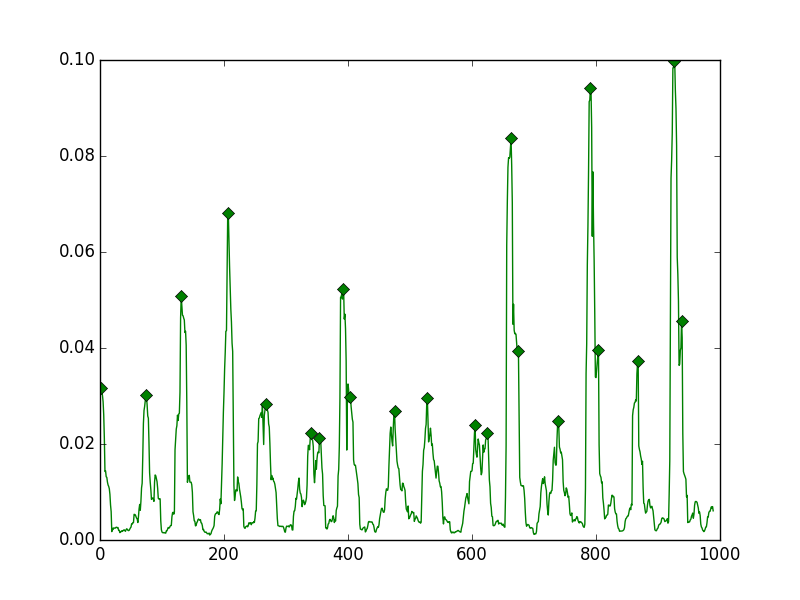
\includegraphics[scale=.50]{figures/608pf}
% \caption{Plot of Bhattacharyya distances for the flight on 6/08/16}
% \label{fig:tamu-fig1}
% \end{figure}

% \begin{figure}[h]
% \centering
% 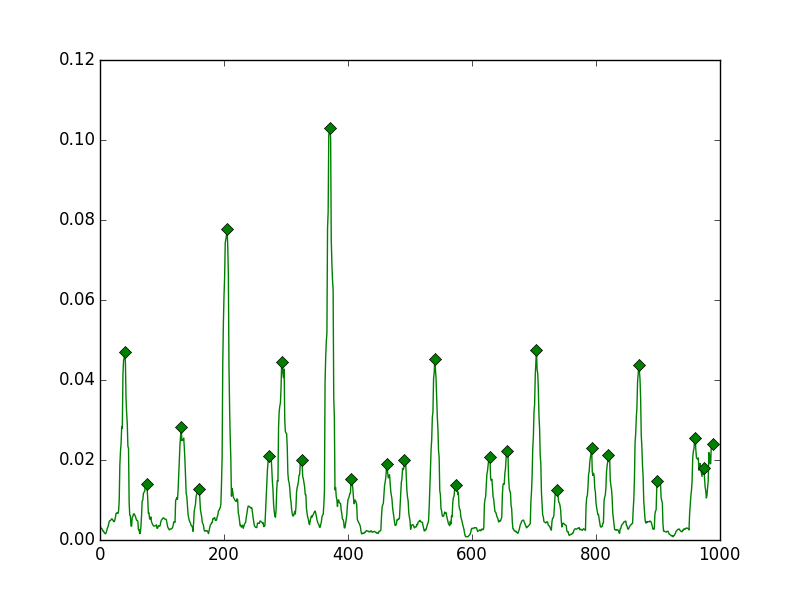
\includegraphics[scale=.50]{figures/629pf}
% \caption{Plot of Bhattacharyya distances for the flight on 6/29/16}
% \label{fig:tamu-fig2}
% \end{figure}

% Between both flight datasets, we achieved a detection rate of 66.0\% and a false alarm rate of 24.1\%.
% While this is not an acceptable level of performance for the system as a whole, it is effective enough to be useful among a set of features used in a training algorithm.
% One reason why this feature does not perform better is that it discards all spatial information in the images; any permutation of the pixels will result in the same pixel distribution.
% Furthermore, this feature alone will perform poorly in distinguishing out-of-sync images that happen to be over a homogeneous area, as the pixel distributions will still be close.


\subsection{Image Feature Descriptors}

As stated, other features are needed in order to create a robust detection system.
From the field of image processing, there are many image features that can be calculated quickly; our goal is to find features which can be compared and matched among consecutive images in a stream to determine if the images are overlapping by the desired amount.
In image processing, keypoints are loosely defined as ``interesting'' parts of an image -- locations in which there is a spike or trough or unique pattern relative to the rest of the image.
The idea with these feature descriptors is to locate a set of keypoints in each image, create descriptors for those points, and then attempt to match them between images to infer that the regions enclosed by matched descriptors are overlapping.

For our feature descriptor extraction, we use corner detection to determine the keypoints used for the descriptors.
An edge in an image is defined as a series of points along which the brightness in an image changes drastically.
Generally, these are located by first finding points at which the brightness changes, and then locating connected components among these points.
A corner, then, is a point at which two edges meet or at which there are two edge directions very close to a point in an image.


From previous research into image classification using feature descriptiors \cite{anomalyhyper}, we identified the SIFT feature as a potential feature which does incorporae spatial information.
This is a scale-invariant feature transform (SIFT) which can be implemented in real time and easily matched between images using L-2 norm differences.


Further research revealed that the binary robust independent elementary features (BRIEF) would be better suited to our purposes.
First, the BRIEF is calculated in less time than SIFT and performs similarly or better on benchmark tests.
Furthermore, the BRIEF keypoints can be matched between images using a simple Hamming distance, rather than the L-2 norm used for SIFT, which also aids in faster processing.
Finally, although it is considered a disadvantage generally, BRIEF is not scale-invariant like SIFT.
Since a scale change between images would not be expected or acceptable, scale-invariance would only result in false matches for our purposes, so the lack of scale-invariance is an advantage.
The full derivation of BRIEF is both lengthy and irrelevant to our immediate research, so it is not included here.
The BRIEF is obtained by first splitting the image into patches based on keypoints, and performing a set of pairwise intensity tests where the intensity of a smoothed patch is compared to another. 
The BRIEF then consists of a bitstring representing the outcome of all pairwise tests between image patches.

For a given keypoint, there exists a substring of the overall BRIEF that represents the outcome of intensity tests between the corresponding image patch and all other patches.
As stated, matching keypoints between images can then be performed by calculating the Hamming distances between these substrings.
A set of matches for each pair of consecutive images is generated, under the constraint that two matching keypoints cannot be more than 1/4 of the image size apart in their respective locations.
This ensures that keypoints are not matched that violate the requirement of about 75\% overlap in consecutive images.

As a metric for comparing the BRIEFs of two images, we look at both the number of keypoints matched as well as the percentage of total keypoints matched. 
This is slightly different than the distance metrics calculated for other features in that a higher value indicates a higher probability that the images are acceptable, but nonetheless yields a single value comparing two images.


\subsection{Blob Detection}

Blob detection is the process of identifying regions in an image that differ from the surrounding regions.
This is similar to the keypoints and descriptors described in the previous section, but involves a continous group of pixels rather than the single points identified by keypoint or corner detection.
More specifically, in our grayscale setting, blobs represent relatively bright or dark spots in an image.

Blobs can be easily calculated by first convolving the target image with the Gaussian kernel:
\begin{equation*}
g(x, y, t) = \frac{1}{2\pi t}e^{-\frac{x^2 + y^2}{2t}} .
\end{equation*}
Then, the Laplacian of this new image is generated, yielding strong positive values for dark spots and strong negative values for bright spots.
The values are thresholded to detect blobs of a size relative to the size of the original Gaussian kernel.
Multiple scales of kernels are used to detect blobs of varying sizes.
The result for a single image is a set of blob locations and their corresponding radii.

To obtain a distance metric for two consecutive images, the blobs for both images are calculated.
Then, we calculate the difference in number of blobs, as well as the difference in total blob area between the two images.


\subsection{Local Binary Patterns}

Local binary patterns are a method of classifying texture within an image.
Texture, in image processing, refers to the relative smoothness or roughness of a section of an image.
Local binary patterns are a relatively simple way of identifying the texture of a given pixel relative to its immediate neighbors.
For a given pixel, a series of intensity tests are performed, the results of which form a binary string which can be converted to an integer.
Then, a histogram is created based on the frequency of each of these integers in the image.
While simple, local binary patterns and their histograms are used extensively in texture classification of images.

As a distance metric, we use the same distribution distance metrics as the general pixel intensity distributions.


\section{Learning Algorithms}

As stated in the problem formulation, we approach the problem with supervised binary classification in mind.
Classification, as opposed to regression, associates a set of features with one of a number of labels, in the binary case there are only two of these labels.
Supervised learning involves training a model with a set of features and their correct labels.
The model then attempts to learn a set of parameters such that when the training data is passed through, the chosen cost function is minimzed with respect to the correct labels.
More generally, the model attempts to adjust its own parameters to output the correct labels for the training data.
There are a large number of supervised classification algorithms available and well-implemented in a number of languages.
Our goal is to identify a number of these which are fundamentally different in their structure and observe the performance of these algorithms for our task.


\subsection{Logistic Regression}

The first among these is logistic regression: one of the most widely used classification algorithms.
Logistic regression takes a labeled training set of feature vectors $\mathbf{x^{(i)}}$ and corresponding binary labels $\mathbf{y^{(i)}}$.
It then finds $\theta$ to minimze the cost function:
\begin{equation}
J(\theta) = \frac{1}{m} \sum_{i=1}^m\frac{1}{2} \left( h_\theta \left( x^{(i)} \right) - y^{(i)} \right)^2
\end{equation}
where $h_\theta (\cdot)$ is the logistic function defined as $h_\theta(x) = \frac{1}{1+e^{-\theta^Tx}}$.

Minimization of the cost function can be performed a number of ways, but the most common is through the gradient descent algorithm.
Gradient descent works by altering the parameters in the direction of steepest descent at each iteration.
For this, the gradient of the cost function relative to the paramenters is taken, and the parameters are altered in the negative of this direction according to a predetermined step size.
The step size or learning rate should be chosen so that the optimization converges as close as possible to the global minimum, while also considering that smaller step sizes take longer to converge.
The learning rate can also be chosen adaptively at each step so that the steps become smaller as the minimum is approached.

\subsection{Artificial  Neural Networks}

The next learning algorithm selected is the multi-layer perceptron (MLP) artificial neural network (ANN).
An ANN is a highly connected directed graphical model, in which the nodes are separated into layers.
Each node in a given layer is connected directionally to each node in the following layer.
In the first layer, called the input layer, the observation or set of features is input into the nodes.
From here, the information propagates from layer to layer according to the weights of the connections between nodes in each layer.
A weighted linear summation is calculated using these weights, which is then passed to a non-linear activation function, such as the hyperbolic tangent function.


In training, the output at the final layer is compared to the desired output, and connection weights are adjusted according to the error through a process called backpropagation.
Starting at the output node, the error is calculated for the training set, and using a gradient descent, similar to that in logistic regression, the weight can be adjusted according to a learning rate and the error times the derivative of the non-linear activation function.
For the hidden layers preceding the output nodes, a similar process is performed by propagating the error at the output layer back to the preceding layer, essentially evaluating the contribution of each node in this layer to the output error.
A gradient descent is then performed in order to update the weights in this layer, followed by propagating these errors back to the preceding layer.
This process is repeated until all hidden layers have been updated, at which point another iteration of the whole process is performed until a minimum is achieved.


ANNs have massive potential for performing at tasks which are difficult to define or explicity program, but often require a large amount of training data and time to become effective.
Multi-layer perceptron networks have the advantage of being able to learn non-linear models, but suffer from a sensitivity to feature scaling and non-unique minima.
As with other ANNs, MLPs may require a great deal of tuning of hyperparameters such as the size and the number of layers.

The typical neural network diagram is displayed below for clarity.

\begin{figure}[htb]
\centering
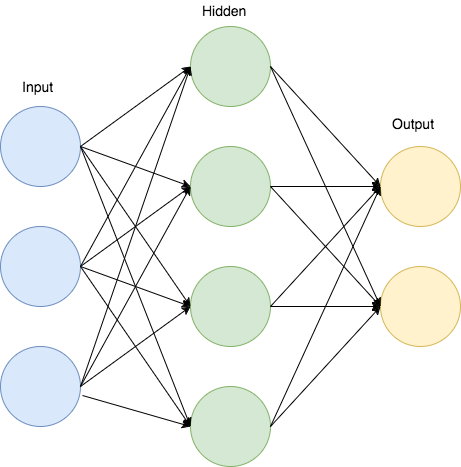
\includegraphics[scale=.50]{figures/NN}
\caption{A general ANN}
\label{fig:tamu-fig3}
\end{figure}


\subsection{Decision Trees}

Another classification algorithm considered is the decision tree. 
A decision tree takes a labeled training set of feature vectors $\mathbf{x^{(i)}}$ and corresponding binary labels $\mathbf{y^{(i)}}$, and finds a set of ordered thresholds to compare the features to in order to classify the vector.
The model is visualized as a binary tree in which one starts at the root node and propagates towards the leaf nodes, which contain classification labels.
Each node in the tree represents a threshold or set of thresholds on a set of features, and the child node is selected based on the comparison of the given features to the thresholds.

These thresholds are calculated based on the training data and a simple greedy algorithm which attempts to minimize the Gini impurity of the following layer of nodes.
The Gini impurity of a set of training examples in a node is a measure of how likely an element of that set is to be mislabeled.
If a set of examples contains $n$ classes, then consider $f_i$ to be the percentage of elements in that set with label $i$.
The Gini impurity can then be expressed as $\sum_{i \not = k} f_if_k$ .

Decision trees are likely the simplest classification algorithm explored in this research, but may perform well if the structure of the problem is simple as well.
The decision tree provides a good point of comparison for the other chosen learning algorithms.

% By comparing the performance of these algorithms, along with the previously mentioned peak-finding, with the image features desired, we believe we can gain a better understanding of the performance of different learning algorithms for this problem, while simultaneously creating a useful system for our intended application.


\subsection{Support Vector Machines}

Support vector machines (SVMs) are the final classification algorithm explored.
An SVM model represents the feature vectors or examples as points in space, such that the points can be separated by a hyperplane to classify the examples as belonging to one category or another.
If the examples are linearly seperable, then a maximum margin hyperplane is genearated by finding two parallel hyperplanes with a maximum distance between them such that the examples are still separated, and taking the parallel hyperplane directly in between these two planes.
In the non-linearly separable case, a hinge loss function is calculated as the sum of distances of incorrectly labeled exmaples to the hyperplane.

The optimal hyperplane is found by first parametrizing the hyperplane as $f(x) = \beta_0 + \beta^Tx$ subject to $|\beta_0 + \beta^Tx| =1$ where $\beta$ is the scale, and $\beta_0$ is the bias.
Then, the distance between each point $x$ and a given hyperplane can be calculated as $\frac{f(x)}{||\beta||}$, which can then be minimized by a number of methods.



\section{Testing Methodology}

The testing methodology for this problem has multiple steps.
First, a subset of the dataset is chosen for testing and evaluating the individual features.
All features and distance metrics are calculated for the pairs of consecutive images in the feature testing subset.
For each feature, the standard deviation of the resulting distance metrics is calculated to ensure that the feature provides a sufficient amount of information.
Next, a graph of these distance metrics is compared to a plot of the labels of the feature testing subset.
The visual comparison of these plots is utilized to determine whether the feature provides some level of distinction between acceptable and anomalous image pairs.

Once the features have been evaluated, and a subset of the features and distance metrics has been selected to use in the learning algorithms, all labeled feature vectors are concatenated.
The data is then split into an 80\% training set and a 20\% testing set.
Each selected learning algorithm is then iteratively trained, tested, and tuned.
Synthetic features, or non-linear combinations of existing features are added and tested for their contribution to performance.
Since most of the learning algorithms explored here operate in a linear fashion, the addition of non-linear combinations can provide a pseudo non-linearity to the algorithms that has the potential to increase performance drastically.
Tuning each learning algorithm involves adjusting the hyperparameters of the model in an attempt to achieve a higher detection rate or lower false-alarm rate.
Depending on the algorithm, this may involve adjusting class weights, learning rate, iterations, number of layers, etc., which is detailed in the following results section.

Finally, the data is split randomly several times into training and testing sets through random resampling or bootstrapping, and the testing scores averaged to obtain a realistic score of performance for each algorithm given the datasets.

